

\documentclass[12pt]{article}
\usepackage[paper=a4paper,left=20mm,right=20mm,top=30mm,bottom =30mm]{geometry}
\usepackage[T1]{fontenc}
\usepackage[utf8]{inputenc}
\usepackage{stmaryrd}
\usepackage{setspace}
\usepackage{mathrsfs}
\usepackage[ngerman]{babel}
\usepackage{amssymb}
\usepackage{amsmath}
\usepackage{enumitem}
\usepackage[colorlinks,linkcolor=black]{hyperref} 
\usepackage{fancyhdr}
\usepackage{subcaption}
\usepackage{graphicx}
\usepackage{lipsum}
\usepackage{float}
\usepackage{color}
\usepackage{listings}


\usepackage{listings}
\usepackage{color}
\usepackage{hyperref}
\usepackage{longtable}
\hypersetup{
     colorlinks   = true,
     citecolor    = gray,
     linkcolor    = blue,
     urlcolor     = blue,
}

\definecolor{mygreen}{rgb}{0,0.6,0}
\definecolor{mygray}{rgb}{0.5,0.5,0.5}
\definecolor{mymauve}{rgb}{0.58,0,0.82}

\lstset{ %
  backgroundcolor=\color{white},   % choose the background color; you must add \usepackage{color} or \usepackage{xcolor}
  basicstyle=\small,        % the size of the fonts that are used for the code
  breakatwhitespace=false,         % sets if automatic breaks should only happen at whitespace
  breaklines=true,                 % sets automatic line breaking
  captionpos=b,                    % sets the caption-position to bottom
  commentstyle=\color{mygreen},    % comment style
  deletekeywords={...},            % if you want to delete keywords from the given language
  escapeinside={\%*}{*)},          % if you want to add LaTeX within your code
  extendedchars=true,              % lets you use non-ASCII characters; for 8-bits encodings only, does not work with UTF-8
  frame=single,	                   % adds a frame around the code
  keepspaces=true,                 % keeps spaces in text, useful for keeping indentation of code (possibly needs columns=flexible)
  keywordstyle=\color{blue},       % keyword style
  language=VHDL,                 % the language of the code
  otherkeywords={*,...},           % if you want to add more keywords to the set
  numbers=left,                    % where to put the line-numbers; possible values are (none, left, right)
  numbersep=5pt,                   % how far the line-numbers are from the code
  numberstyle=\tiny\color{mygray}, % the style that is used for the line-numbers
  rulecolor=\color{black},         % if not set, the frame-color may be changed on line-breaks within not-black text (e.g. comments (green here))
  showspaces=false,                % show spaces everywhere adding particular underscores; it overrides 'showstringspaces'
  showstringspaces=false,          % underline spaces within strings only
  showtabs=false,                  % show tabs within strings adding particular underscores
  stepnumber=1,                    % the step between two line-numbers. If it's 1, each line will be numbered
  stringstyle=\color{mymauve},     % string literal style
  tabsize=2,	                   % sets default tabsize to 2 spaces
  linewidth=15cm,
  title=\lstname                   % show the filename of files included with \lstinputlisting; also try caption instead of title
}

\usepackage{caption}
\captionsetup[lstlisting]{font={scriptsize}}
\DeclareGraphicsExtensions{.pdf,.png,.jpg}

\pagestyle{fancy}
\lfoot{Carl Schaffer}
\rfoot{carl.schaffer@cern.ch}
\cfoot{-\thepage-}
\renewcommand{\headrulewidth}{0.6pt}
\renewcommand{\footrulewidth}{0.6pt}
\setlength{\headheight}{37pt}
\setlength{\parindent}{0pt}
\renewcommand{\familydefault}{\sfdefault}

\newcommand{\exercise}[2]{\section{#1}\hfill{}\\}

\newcommand{\doublefig}[2]{\begin{center}
  \begin{tabular}{ll}
    a.) &b.)\\
    \includegraphics[width=.3\textwidth]{#1}&  \includegraphics[width=.3\textwidth]{#2} 
  \end{tabular}
\end{center}
}

\newcommand{\doublefignolabel}[2]{\begin{center}
  \begin{tabular}{ll}
    \includegraphics[width=.2\textwidth]{#1}&\includegraphics[width=.3\textwidth]{#2}
  \end{tabular}
\end{center}
}


\newcommand{\signal}[1]{\texttt{#1}}
\newcommand{\stdl}{\lstinline$standard_logic$}
\newcommand{\stdlv}[2]{\lstinline$standard_logic_vector(#1 downto #2)$}
\newcommand{\vhdl}[1]{\lstinline$#1$}
\newcommand{\loghi}{\vhdl{'1'}}
\newcommand{\loglo}{\vhdl{'0'}}

\newcommand*{\bashcode}{\lstinline[{language=[LaTeX]TeX}]}
\newcommand{\bash}[1]{\bashcode$#1$}
\newcommand{\git}{\texttt{GIT}}

\newcommand{\nandGate}{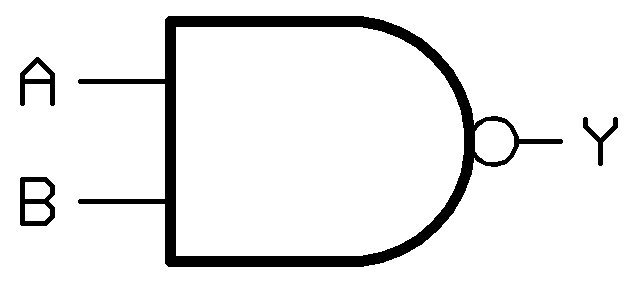
\includegraphics[width=3cm]{./images/nand}}
\newcommand{\andGate}{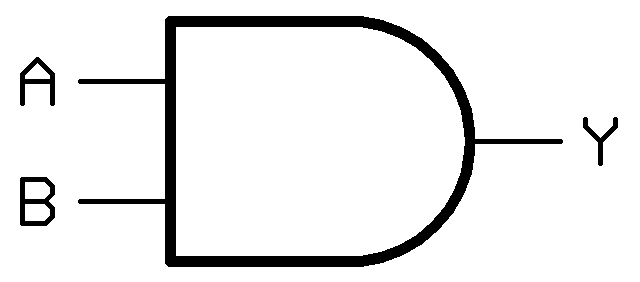
\includegraphics[width=3cm]{./images/and}}
\newcommand{\notGate}{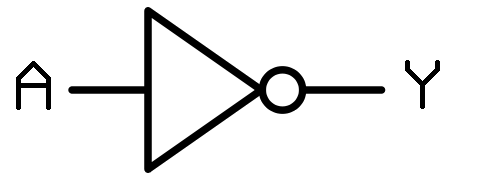
\includegraphics[width=3cm]{./images/not}}
\newcommand{\xorGate}{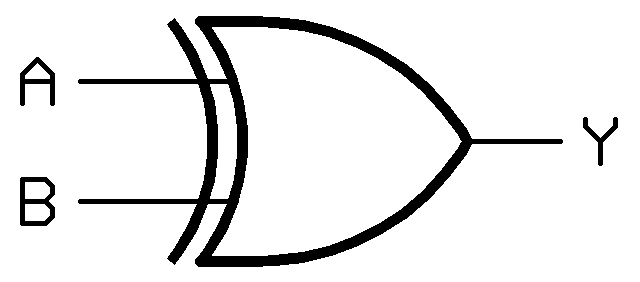
\includegraphics[width=3cm]{./images/xor}}
\newcommand{\orGate}{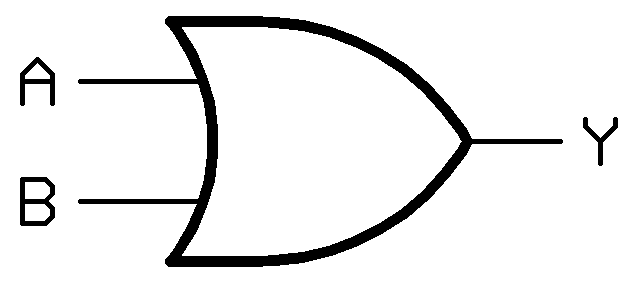
\includegraphics[width=3cm]{./images/or}}

\newcommand{\ise}{XILINX ISE}

\newcommand{\al}[1]{
\begin{align}
#1
\end{align}
}


\newcommand{\pic}[2]{\begin{center}\includegraphics[width=#1\linewidth]{#2}\end{center}}

\newcommand{\nn}{\nonumber}

\newcommand{\lr}[1]{
\left( #1 \right)
}

\newcommand{\head}[3]{%
\pagestyle{empty}

\vspace{-1.5cm}
\noindent Albert-Ludwigs-Universität Freiburg \hfill SS #1\\
\hrule

\begin{center}
  \section*{Übungsblatt #2}
  \large zur Vorlesung \textit{Einführung in die moderne Digitalelektronik} \normalsize \\
  \vspace{0.5cm}
  Prof. Dr. Horst Fischer, #3\\
\end{center}
\hrule
\vspace{0.5cm}
}


\fancyhead[R]{{\large \textbf{Blatt 3}}}


\begin{document}
\head{2021}{3}{Daniel Baur}




%------------------------------------------------------
%------------------------------------------------------
\part*{Erste Schritte in VHDL}
%------------------------------------------------------
%------------------------------------------------------


%Ziel dieser Übungen ist die Implementierung einer Stoppuhrschaltung
Im Rahmen dieses Übungsblockes
\vspace*{-5pt}
\begin{itemize}
    \setlength\itemsep{-5pt}
    \item werden einzelne Logikgatter-Module in VHDL programmiert
    \item und in eine komplexere Schaltung implementiert,
    \item welche anschließend auf einem FPGA-Chip synthetisiert werden soll.
\end{itemize}


Laden Sie sich dazu das Projekt
\texttt{erste\_schritte\_in\_vhdl\_\_vorlage.tar}
von der Adresse \url{https://ilias.uni-freiburg.de/goto.php?target=file_1738699_download&client_id=unifreiburg} (Ilias Seite)  herunter.
Nach der Übung werden auch Lösungsvorschläge auf ILIAS veröffentlicht.





%------------------------------------------------------
\exercise{ISE starten}{-1}
%------------------------------------------------------


Machen Sie sich mit dem \textit{Command Line Interface} (\textit{CLI}, \textit{Terminal}) der auf dem CIP-Pool-Rechner installierten Linux-Distribution vertraut. Starten Sie dann die \textit{ISE Design Suite} indem Sie entweder


\begin{itemize}
\setlength\itemsep{-25pt}


\item ein Terminal öffnen und die folgenden Befehle ausführen,
\begin{lstlisting}[language=bash]
cd /mnt/ISE/14.7/ISE_DS
export XILINXD_LICENSE_FILE=2100@license.physik.privat
source settings64.sh
ise
\end{lstlisting}
\vspace*{-1mm}


\item oder ein entsprechendes \texttt{bash}-Skript erstellen.


\end{itemize}





%------------------------------------------------------
%------------------------------------------------------
\exercise{Programmieren von kombinatorischer Logik in VHDL}{1}
\label{gates}\noindent 
%------------------------------------------------------
%------------------------------------------------------


Programmieren Sie die folgenden Gatter in VHDL.
Vervollständigen Sie dazu zunächst das im Projekt bereits vorhandene And-Gatter und dessen
testbench im tb Ordner. Simulieren Sie daraufhin zunächst das And-Gatter mit Isim.
Legen Sie nun für jedes der weiteren Gatter in gleicher Weise eine Entity für das Gatter und dessen
Simulation an und fügen diese .vhdl files zum Projekt hinzu. Simulieren Sie daraufhin alle Gatter.


\begin{center}
  \begin{tabular}{ccccc}
    a.)&b.)&c.)&d.)&e.)\\
    \andGate&\orGate&\notGate&\xorGate&\nandGate\\
    \texttt{AND}&\texttt{OR}&\texttt{NOT}&\texttt{XOR}&\texttt{NAND}\\
  \end{tabular}
\end{center}
%\clearpage
\exercise{Verketten von kombinatorischer Logik in VHDL}{2}


In dieser Aufgabe sollen VHDL Module verkettet und mit dem Ergebniss einer direkten logischen Zuweisung verglichen werden. Die Entities für die beiden folgenden Aufgabenteile sind bereits als
schaltung\_a.vhd und schaltung\_b.vhd im Projekt vorhanden.


\begin{enumerate}[label=\alph*.)]


\item Implementieren Sie folgende Schaltung mit Hilfe der in
  Aufgabe \ref{gates} erstellten Entities.
  \begin{center}
    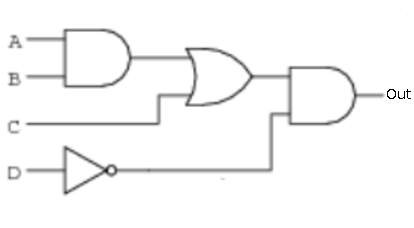
\includegraphics[width= 7cm]{./images/01301x01}
  \end{center}
\vspace*{-25pt}
Vervollständigen Sie dazu die im Projekt bereits vorhandene Datei schaltung\_a.vhd.


\item Implementieren sie nun die selbe Funktionalität mithilfe der VHDL Signaloperatoren
  \texttt{and}, \texttt{or}, \texttt{nand}, \texttt{nor}, \texttt{xor}, \texttt{not}.
 indem Sie eine einzelne Signalzuweisung nutzen.
 Vervollständigen Sie dazu die Datei schaltung\_b.vhd.


\item Simulieren Sie die beiden Module, indem Sie zunächst die Datei testbench\_schaltung.vhd
vervollständigen und daraufhin das Ergebniss mit Isim betrachten.


\end{enumerate}





%------------------------------------------------------
\exercise{Ein erstes Leuchten}{3}
%------------------------------------------------------


In dieser Aufgabe werden Sie schaltung\_a oder schaltung\_b in der Hardware testen.


\begin{enumerate}[label=\alph*.)]


\item Nutzen Sie das Handbuch zum Spartan 3 Starter Kit (\href{https://www.xilinx.com/support/documentation/boards_and_kits/ug130.pdf}{UG130}) um das file signal\_mapping.ucf
zu vervollständigen.


\item Vervollständigen Sie die Datei toplevel.vhd. Die Eingänge von vier unterschiedlichen switches
am Spartan Board sollen auf die Eingänge von schaltung\_a oder schaltung\_b gegeben werden
und der Ausgang der Schaltung auf eine beliebige LED.


\item Erstellen Sie eine Binärdatei des Designs und laden Sie diese in den Spartan FPGA.
Überprüfen Sie, ob beim Umlegen der richtigen switches daraufhin die LED korrekt an- bzw.
ausgeht.


\item Bonus: Bringen Sie alle LEDs zum Leuchten, wenn das Ergebniss von schaltung\_a oder schaltung\_b wahr ist. Nutzen Sie hierzu die others Anweisung.


\end{enumerate}





%------------------------------------------------------
%------------------------------------------------------
\part*{Die Stoppuhr}
%------------------------------------------------------
%------------------------------------------------------


Das Ziel dieser Übungen ist die Realisierung einer Stoppuhrschaltung.\\

Laden Sie sich dazu von der Adresse \url{https://ilias.uni-freiburg.de/goto.php?target=file_1740380_download&client_id=unifreiburg}
das .tar-file \texttt{die\_stoppuhr.tar} herunter, entpacken Sie es und laden das Projekt in ISE DS. Alle benötigten VHDL-Module sind in diesem Projekt bereits angelegt.\\

\textit{Hinweis}: Bitte löschen Sie am Ende der Übung die großen Dateien im Ordner \texttt{./ise/}!





%------------------------------------------------------
\exercise{BCD Zähler}{1}
%------------------------------------------------------


Wir wollen einen dezimalen (\textit{binary coded decimal}) Zähler programieren der von 0 bis 9999 zählt.
Betrachten Sie dazu das Modul \textit{bcd\_counter}. Der 16 bit breite Ausgang \textit{BCD\_OUT} soll dabei als vier Worte aus jeweils 4 bit aufgefasst werden. Jedes dieser Worte representiert eine Ziffer zwischen 0 und 9 und die vier Worte representieren gemeinsam den Zählerstand im Dezimalsystem.


\begin{enumerate}[label=\alph*.)]


\item Vervollständigen Sie das Modul \textit{bcd\_counter}, so dass bei jedem \textit{CLK\_en} der Wert des Ausgangs \textit{BCD\_OUT} nach obiger Auffassung um eins erhöht wird.


\item Implementieren Sie ein asynchrones reset, welches den Zählerstand auf null setzt, sobald der
Eingang \textit{RST} den Wert logisch eins annimmt.


\item Verifizieren Sie das Modul mit Hilfe der Testbench \textit{tb\_bcd\_counter}. 


\end{enumerate}


\textit{Bemerkung}: Ignorieren Sie für den Moment den Eingang \textit{start\_stop} und das Signal \textit{was\_stopped}. Den Vektor \textit{BCD\_OUT} können Sie etwa mithilfe von \glqq \texttt{BCD\_OUT (3 downto 0)}\grqq \,\,komponentenweise referenzieren.





%------------------------------------------------------
\exercise{Taktskalierung}{1}
%------------------------------------------------------


Machen Sie sich die Aufgabe und Funktionsweise des Moduls \textit{scale\_clock} klar.


\begin{enumerate}[label=\alph*.)]


\item Lesen Sie den Code und simulieren Sie das Module mit Hilfe der Testbench \textit{tb\_clock\_scaler}.


\item Auf welchen Wert muss der generic \textit{limit} gesetzt werden, damit man bei
einem eingehenden 50\,MHz Takt einen Abstand zwischen den einzelnen \textit{CLK\_10HZ\_enable} Signalen von 0,1\,s hat?


\end{enumerate}





%------------------------------------------------------
\exercise{Das Seven-Segment LED Display}{1}
%------------------------------------------------------


Machen Sie sich mit Hilfe des Spartan-3 User Guides (\href{https://www.xilinx.com/support/documentation/boards_and_kits/ug130.pdf}{UG130}) die Funktionsweise des Seven-Segment LED Displays
klar.


\begin{enumerate}[label=\alph*.)]


\item Vervollständigen Sie das Modul \textit{seven\_seg\_encoder}, so dass eine nicht vorzeichen-
behaftete 4 bit Zahl in hexadezimaler Schreibweise auf dem Display angezeigt werden kann.


\item Verifizieren Sie das Modul mit Hilfe der Testbench \textit{tb\_seven\_seg}.


\item Machen Sie sich mit Hilfe des User Guides mit dem ein und Auschalten der vier Display Segmente
und dem Dezimalpunkt vertraut. Vervollständigen Sie das Modul \textit{display\_controller} 
dessen Aufgabe es ist durch korrekte Bedienung der Steuersignale \textit{LED\_OUTPUT}, \textit{DISABLE\_LED} und \textit{DECIMAL\_POINT} einen Zählerstand \textit{COUNTER\_INPUT} auf dem Display darzustellen. Nutzen Sie hierzu das Modul 
\textit{seven\_seg\_encoder} und lassen sie für eine geeigneten Anzahl an Taktzyklen jeweils
eines der Display Segmente eingeschaltet (Stichwort Multiplexing). Hierzu müssen Sie einen einfachen Zähler innerhalb eines
getakteten Prozesses nutzen.


\item Nutzen Sie die Testbench \textit{display\_controller\_tb} um das Modul zu verifizieren.


\end{enumerate}





%------------------------------------------------------
\exercise{Projekt: Eine erste Stoppuhr}{1}
%------------------------------------------------------


Instanzieren Sie die Module \texttt{scale\_clock.vhd}, \texttt{bcd\_counter.vhd} und \texttt{display\_controller.vhd} im toplevel.
Verbinden Sie dann die Module auf geeignete Weise, sodass auf dem Display eine dezimale Stoppuhr angezeigt wird, welche in Schritten von $0.1\,\mathrm{s}$ hochzählt und durch Drücken eines der Buttons resertiert werden kann.
Erstellen sie abschließend das Binärfile und konfigurieren Sie den FPGA um ihr Design in der Hardware zu testen.





%------------------------------------------------------
\exercise{Bonus: Eine bessere Stoppuhr}{1}
%------------------------------------------------------


Die Stoppuhr soll nun dahingehend verbessert werden, dass mit dem Betätigen eines weiteren Buttons die Stoppuhr angehalten und bei erneutem Drücken desselben Buttons weiter laufen gelassen wird:


\begin{enumerate}[label=\alph*.)]


\item Vervollständigen Sie das Modul \texttt{debouncing.vhd} indem Sie einen Zähler innerhalb eines getakteten Prozesses nutzen um einen Button zu entprellen. Simulieren Sie das Modul mit der Testbench \texttt{tb\_debouncing.vhd}.


\item Widmen Sie sich nun dem Eingang \textit{start\_stop} des Moduls \texttt{bcd\_counter.vhd}:\\
Implementieren Sie mithilfe des Signals \textit{was\_stopped} ein Stoppen und Starten des Zählers falls der Eingang \textit{start\_stop} auf eins wechselt. Simulieren Sie das Modul erneut mit der Testbench \texttt{tb\_bcd\_counter.vhd}.


\item Instanzieren Sie das Modul \texttt{debouncing.vhd} im Toplevel unter geigneter Verbindung mit einem Button und dem Modul \texttt{bcd\_counter}, so dass das Ziel der Aufgabe erreicht wird und testen Sie ihr Ergebniss in der Hardware.


\end{enumerate}


\textit{Bemerkung}: Konsequenterweise sollte man nun auch den Reset-Button auf ein weiteres Debouncing-Modul geben und alle asynchronen resets im Design durch synchrone ersetzen. Ein asynchrones Reset birgt immer eine kleine Gefahr...
















\end{document}















